\newpage

%Introduction
%Time-independent reliability analysis
%  - Formulation (general context)
%  - challenges and methods (low failure probabilities, high-dimensionality, costly to evaluate), (simulation based, approx based, and hybrid)
%Time-dependent reliability analysis
%  -From static to time-dependent
%  -Challenges and review of methods
%  -Proposed method
%   - idea (time-depenednt to system)
%   - AK-SYS 
%   - AK-SYS-T
%ù   - Validation and case studies
%Conclusion

\section{Introduction}
\noindent
It was well elucidated in previous chapter that a proper assessment of structural performance will lead to a better optimal planning of interventions to extend the 
service life of existing structures. Performance indicators provide a measure to evaluate the deterioration of structural performance through time. With this 
respect time-dependent reliability can be employed to provide a well-suited indicator for structural LCM against fatigue. It enables to take into account the 
associated uncertainties in the phenomenon and provides an estimation of cumulative failure probability for a given time interval. Having the time as an input
parameter amplifies the difficulty of dealing with reliability problems. One challenge in this domain is dealing with non-monotonic performance functions especially 
when the performance function is costly-to-evaluate. Therefore, the goal of this chapter is to propose a new time-dependent reliability method which tries to tackle this 
issue. 

The new methodology is called AK-SYS-T. The idea behind this method is to relate the time-dependent reliability problems with system reliability problems to be able to 
take advantage of efficient system reliability methods. This can be dome by discretizing the desired time interval into a finite number of time nodes. AK-SYS is a recently 
developed efficient system reliability method. In this method, performance functions for components are replaced with Kriging meta-models and an active learning process is 
used for the enrichment of the Design of Experiments (DOE). AK-SYS owes its efficiency to its learning process owing to the fact that it only searches among the most vulnerable 
components to update the DOEs. This learning process is used towards time-dependent reliability problems and the result is AK-SYS-T. This method is introduced in this chapter. 

Accordingly, the rest of this chapter is organized as follows. 

\section{Time-independent reliability analysis}
\noindent
The main goal of structural reliability analysis is to find the probability of failure under given conditions and for a given period of time. In reliability analysis, failure does
not refer to the structural failure (such as structural collapse) only. In most cases, failure is defined as a situation when the structural performance exceeds a given threshold. 
The concept of limit state is therefore employed to define the failure. Generally, two types of limit states can be realized for structures: 1) ultimate limit states and 2) 
serviceability limit states. Failure modes within the former limit states are related to the loss of load carrying capacity such as weld rupture, fatigue rupture, formation of
plastic hinge, etc. The latter limit states include failure modes related to gradual deterioration, user's comfort, etc. Undesired deflections, corrosion, and excessive deformations
are some examples of the failure modes related to serviceability limit states. 

Structural reliability problem are generally formulated by a so called performance function. As mentioned before, a "stress-strength" approach is used to define the structural 
performance function. Considering only one load effect $Q$ and one resistance $R$, the basic form of the performance function can be formulated as $G=R-Q$. For many problems it 
is not feasible to reduce the structural performance function to a simple formulation of $R$ versus $Q$. By considering all the basic variables $\textbf{X}$ involved in the problem,
$R$ and $Q$ can be expressed as $R=G_R(\textbf{X})$ and $Q=G_Q(\textbf{X})$ respectively. In this way, the resulting performance function can be written in a general form as
$G(\textbf{X})$ where $G()$ is a function that expresses the structural performance as a relationship between basic variables. The equation $G(\textbf{X})$ defines the limit state 
which is the boundary between the safe domain $G(\textbf{X})>0$ and the failure domain $G(\textbf{X})<0$. Different concepts in structural reliability analysis are illustrated in 
Figure \ref{fig:fail-domain}.

\begin{figure*}[hbt!]
\centering
  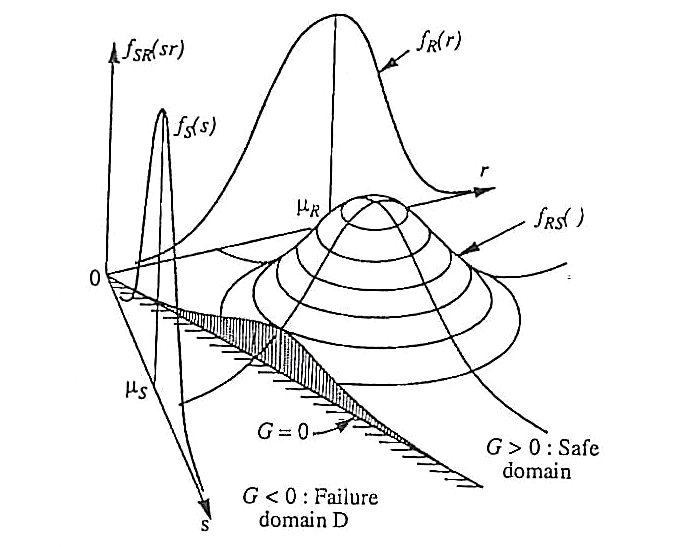
\includegraphics[width=0.7\linewidth]{figures/fig-ch2/limit-state-violation.png}
  \caption{An illustration of different concepts in reliability analysis: failure domain $G<0$, safe domain $G>0$, limit state $G=0$, joint density function $f_{rs}()$, 
  and marginal density functions $f_r()$ and $f_s()$}
  \label{fig:fail-domain}
\end{figure*}

Given the general form of the performance function $G(\textbf{X})$, the failure probability can be calculated by integrating the the joint probability density function 
$f_{\textbf{X}}(\textbf{x})$ of n-dimensional vector $\textbf{X}$ of the basic variables over the failure domain $G(\textbf{X})<0$ (see Equation \ref{eqation:t-in-rel}). 

\begin{equation}
P_f = P(G(\textbf{X})<0) = \int ... \int_{G(\textbf{X})<0}f_{\textbf{X}}(\textbf{x})d\textbf{x}
\label{eqation:t-in-rel}
\end{equation}
\noindent
Given that the basic variables are independent, the joint probability density function can be simplified as: 
\begin{equation}
f_{\textbf{X}}(\textbf{x})= \prod_{i=1}^{n}f_{x_i}(x_i)
\label{eqation:density}
\end{equation}
where $f_{x_i}(x_i)$ denotes the marginal density function for the basic variable $X_i$. 



\section{General context of reliability analysis}
\noindent
As said before, structural reliability is defined over a given period of time and it tries to evaluate the probability that a structure accomplishes its intended 
duties under specified conditions by taking into account the uncertainties associated with material properties, geometry, and loading. Performing structural reliability 
analysis requires a performance function $G$ that take into account the effect of all uncertainties as input. The basic form of the performance function is based on 
"stress-strength" definition as mentioned in \ref{subsec:fatigueperformance}. The performance function hence can be formulated as $G = R-Q$ in which $R$ and $Q$ represent
respectively the resistance capacity (strength) and the load effect (stress). Accordingly, a limit state $G=0$ can be defined to separate the failure domain $G<0$ from 
the safe domain $G>0$. 

In real world cases, structural performance function can be a time dependent process (such as the performance functions for fatigue in Section \ref{subsec:fatigueperformance})
that is associated with a set of random variables $\textbf{X}$ (e.g. material properties, geometry, etc.) and a set of stochastic processes $\textbf{Y(t)}$ (such as service and
environmental loading, wind velocity, etc.). Therefore, the general form of the performance function can be represented as $G(\textbf{X}, \textbf{Y}(t), t)$. Dealing with time 
is an important issue in reliability analysis since it introduces extra complexity to the problem. For this reason, reliability problems can be categorized in two groups:
1- time-independent and 2- time-dependent problems. 


Methods in the first group try to find the failure probability at a give time instant $t_i$ as it is formulated in Equation
\ref{eq:inst}. 
\begin{equation}
P_{f,i}(t_i) = \textrm{Prob}(G(\textbf{X},\textbf{Y}(t_i), t_i) \leq 0)
\label{eq:inst}
\end{equation}

Methods in the second group, however, try to deal with the complete aging process and loading history for a given time interval $[t_0, t_l]$. Therefore, the aim
of time-dependent reliability methods is to find the cumulative failure probability which is defined as: "the probability of having at least one failure during a given time 
interval $[t_0,t_l]$", see Equation \ref{eq:cum}. Figure \ref{fig:cum-inst} illustrates the differences between these two failure probabilities. 
\begin{equation}
P_{f,c}(t_0,t_l) = \textrm{Prob}(\exists\tau \in [t_0, t_l] , G(\textbf{X},\tau) \leq 0)
\label{eq:cum}
\end{equation}

\begin{figure*}[hbt!]
\centering
  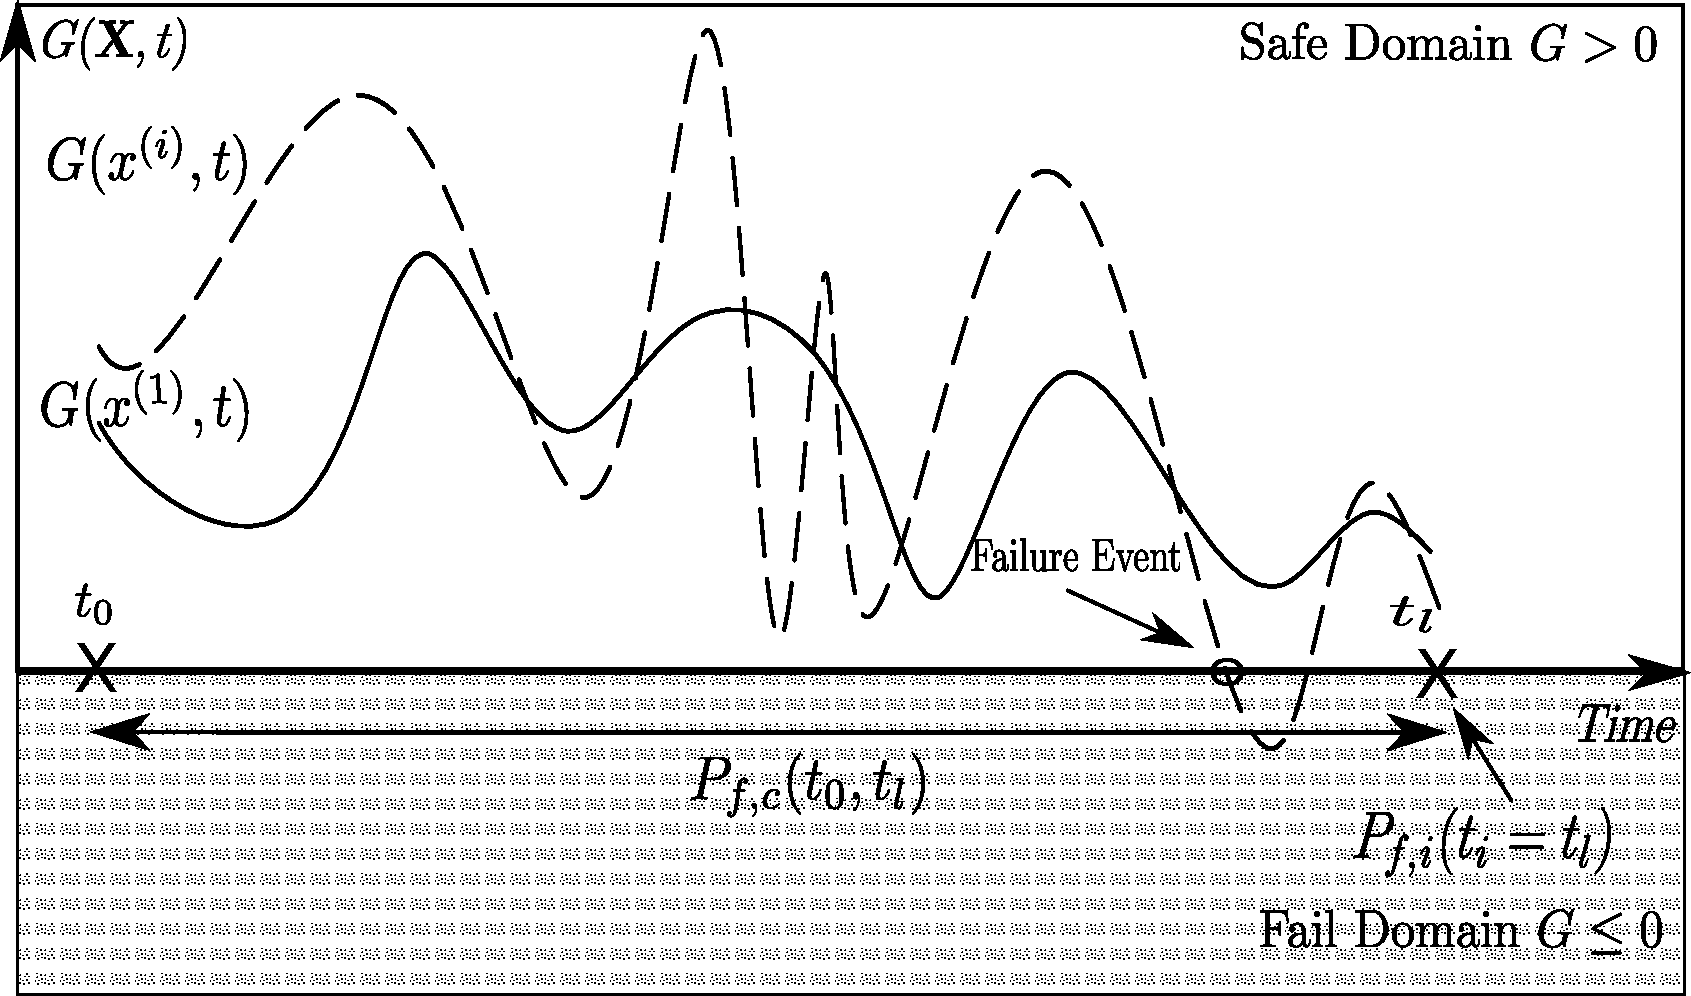
\includegraphics[width=0.75\linewidth]{figures/fig-ch2/performanceink.pdf}
  \caption{An illustration of instantaneous and cumulative probability of failure}
  \label{fig:cum-inst}
\end{figure*}


\subsection{Time-independent reliability analysis and methods}
\subsection{Time-dependent reliability analysis and methods}


\noindent
Time adds extra complexity to the problem. Compared to the time-independent problems, the limit state in time-dependent reliability is changing by time and one should 
also consider the complete aging process and load history of a structure. The general form of the performance function for a time-dependent reliability problem can be 
expressed as $G(\textbf{X},\textbf{Y}(t),t)$ where $\textbf{Y}(t)$ is the vector of input random processes. Random processes can be decomposed into random variables
using some appropriate random process representations such as Karhunen-Loeve (KL) expansion \citep{Loeve1977} or spectral representation method \citep{Chun1993}. 
Therefore, the performance function can be represented by $G(\textbf{X},t)$ for the rest of this study. The parameter of interest in time-dependent reliability 
analysis is to find the cumulative probability of failure $P_{f,c}(t_0,t_l)$ (see Equation \ref{eq:cum}). Calculating this failure probability is, in principle, 
possible using sampling methods such as crude MCS, importance sampling, etc. However, the computational cost of using MCS for time-dependent reliability problems is 
enormous which makes this method useless in 
the time-dependent context. The challenge in time-dependent reliability methods is to achieve a reasonable trade-off between efficiency and accuracy especially for the 
problems with non-monotonic performance functions that are costly-to-evaluate and have high dimensionality. Available methods for time-dependent reliability analysis 
can be categorized into two groups: out-crossing-based methods and extreme-value-based methods. Methods in the second category can provide a better accuracy, however, 
computational cost in the first category is lower. These methods will be briefly reviewed in Section \ref{sec:methods}. 

In most of time-dependent reliability methods, discretizing the time interval of interest into a finite number of time nodes is the main strategy to tackle the 
complexity that is added to the problem by time parameter. In addition to time, input stochastic processes must be discretized. This is a bit more complicated
since it needs to approximate a stochastic process with a combination of some random variables and explicit functions of time. In this way the process uncertainty can
be separated from its time dependency. After the discretization, one can introduce an instantaneous performance function for each time node, hence, the problem will 
be converted to a time-independent one. Failure at each node implies the failure of whole structure. This is equivalent to finding the probability of failure in a 
serially connected system in which each component represent the time nodes after discretization. This brings the idea to employ efficient system reliability 
methods to address time-dependent reliability problems. Therefore, the goal of this chapter is to present a newly developed time-dependent reliability method that is 
called AK-SYS-T. This method is based on AK-SYS that developed for system reliability analysis using Kriging meta-modeling and an active learning process. AK-SYS is
reviewed is Section \ref{sec:ak-sys}. 

The rest of this chapter is organized as follows: Section \ref{sec:methods} provides a background information about time-dependent reliability assessment and current 
methods in this field. Fill this part after the chapter is finished. 


\section{Background and review of time dependent reliability methods}
\label{sec:TDmethods}

\noindent
Addressing time-dependent reliability problems is always a challenge. Different challenges that need to be addressed in this domain are related to problems with low 
failure probabilities, high dimensionality, complex and computationally expensive performance function, or a combination of them where finding a balance between 
efficiency and accuracy is always pursued. Several methods have already been developed for time-dependent reliability analysis and they can mainly categorized into 
two main groups namely Out-Crossing-Based (OCB) methods and Extreme-Value-Based (EVB) methods. The aim of the methods in the first group is to find the crossing rate
of the performance function from the safe domain to the failure domain while methods in the second group are searching for the extreme value of the performance 
function (the extreme value here refers to the minimum value of the performance function). 

\subsection{OCB methods}

\noindent
The cumulative probability of failure, within the methods in OCB, is linked to the first-time-to-failure or the first passage $t_{f}$. The first-time-to-failure is 
a random variable and it corresponds to the first time instant that the performance function crosses the limit state. The formulation of $P_{f,c}(t_0,tl)$ can be hence
written as: 
\begin{equation}
P_{f,c}(t_0,t_l) = \textrm{Prob}(t_{f}<t_l)
\label{eq:cumcross}
\end{equation}
This equation implies that the cumulative probability of failure within $[t_0, t_l]$ is equal to the probability of having at least one out-crossing event from the 
safe to the fail domain. If $N_{[t_0,t_l]}$ counts the number of out-crossing events within the desired time interval, the previous formulation for cumulative 
probability of failure can be converted to the Equation 
\begin{equation}
P_{f,c}(t_0,t_l) = P(G(\textbf{X},0) \leq 0 \cup N_{[t_0,t_l]} \geq 1)
\label{eqation: cumnew}
\end{equation}
It has been shown that the cumulative failure probability can be bounded such as: 
\begin{equation}
\underset{t \in [t_0, t_l]}{\text{max}}P_{f,i}(t) \leq P_{f,c}(t_0,t_l) \leq P_{f,i}(0)+E[N_{[t_0,t_l]}]
\label{eqation: bound}
\end{equation}
where $E[N_{[t_0,t_l]}$ is the mean value of out-crossing numbers. 
The problem therefore lies in estimating the mean value of out-crossings during the desired period of time $[t_0,t_l]$. This requires the estimation of the 
out-crossing rate $\nu (t)$. The mean value of out-crossings can be formulated by Eq.\ref{eqation: meanoutcross}.
\begin{equation}
E[N_{[t_0,t_l]}] = \int_{t_0}^{t_l}\nu (t)dt 
\label{eqation: meanoutcross}
\end{equation}
Calculating this rate is a complicated task for the methods in this category. If the performance function can be expressed as a stationary and differentiable 
univariate process that is added to a constant threshold, then the Rice's formula can be used to find the out-crossing rate \cite{Rice1944}. Employing Rice's 
formula, analytical formulations of out-crossing rate has been obtained for a stationary Gaussian process in \cite{LUTES20041} and also for a general Gaussian 
process (stationary and non-stationary) in \cite{LUTES2009, Surdet2008}. 

It can be easily shown that the $N_{[t_0,t_l]}$ follows a binomial distribution using some basic probability theories. Binomial distribution tends to be a 
Poisson distribution for long-term reliability assessment. Under this assumption, one can neglect the dependence between the out-crossing events. Therefore, 
the rate for first-time-to-failure is equal to the out-crossing rate \cite{Ponte1985}. The out-crossing rate can be also approximated by sampling techniques 
like importance sampling \cite{Singh2011}. Ignoring the dependency between the out-crossing events for problems with high reliability levels (low probability
of failure) can cause a big amount of error in calculations \cite{Zhang2011, LUTES2009, Surdet2008}. Researchers have tried to mitigate this deficiency by 
using joint out-crossing rates \cite{Hu2013} and first order sampling approach \cite{Hu2015}. 

One of the most popular methods in this category is PHI2 method \cite{ANDRIEURENAUD200475} that is extensively used for its numerical efficiency. This method
is based on system reliability analysis. A parallel system hence is considered for time instant $t$ and $t+\Delta t$. The out-crossing happens if the system is 
in safe domain at time $t$ and in the fail domain at time $t+\Delta t$. Accordingly, the out-crossing rate can be formulated as: 

\begin{equation}
\nu (t)= lim_{\Delta t \to\ 0^+}\frac{Prob((G(t)>0)\cap G(t+\Delta t\leq0))}{\Delta t}
\label{eqation: phi2out}
\end{equation}

PHI2 tries to approximate this out-crossing rate using FORM which is a time-independent reliability method. For this reason, two FORM are used. One to estimate 
the probability of failure associated with $G(t)>0$ and the other one for $G(t+\Delta t\leq0)$. In this method there is no need to discretize the time interval 
the input stochastic processes can be replaced with two random variables $Y(t)$ and $Y(t+\Delta t)$ for time instants $t$ and $t +\Delta t$. 
PHI2 method provides an upper bound for failure probability that causes underestimating the reliability level. The choice of the time increment $\Delta t$ is 
crucial and affects the accuracy of this method. An approximation should be made on the choice of time increment, see \citep{Surdet2008}. For this reason, 
PHI2+ has been proposed in \cite{Surdet2008}. This method is an improvement of the initial PHI2 method that tries to stabilize the effect of the time increment 
$\Delta t$. However, it should be noted that PHI2+ may lead to significant errors in case of highly nonlinear limit states. More recently, a method named mean 
value first passage method has been proposed in \cite{Zhang2011, Du2012} for kinematic reliability applications. Up-crossing rates are derived analytically 
(under simplifying assumptions) and time-dependent reliability can be calculated by integrating those analytical equations. The integration process has been 
done using a numerical procedure proposed in this study. In general out-crossing-based methods use FORM to approximate failure probability. Therefore 
their accuracy for highly nonlinear performance functions is questionable.

\subsection{EVB methods}
\noindent
Methods in this category search for the extreme values of the performance function (global minimum here). The cumulative probability of failure then can be 
defined as the probability that the global minimum of the performance function becomes negative which is formulated in Equation \ref{eqation: complimit}. 

\begin{equation}
P_{f,c}(t_0,t_l) =  P(\underset{t \in [t_0, t_l]}{\text{min}} \; G(\textbf{X},t) \leq0 ) 
\label{eqation: complimit}
\end{equation}
\noindent
Finding the global minimum ($G_{min}$) of the performance function requires the discretization of time and random processes and it is defined as following 
equation.

\begin{equation}
G_{min}(\textbf{X})= \underset{t \in [t_0, t_l]}{\text{min}} \; G(\textbf{X},t) \leq0 ) 
\label{eqation: globalmin}
\end{equation}

\noindent
$G_{min}$ is a random variable and the cumulative probability of failure can be accurately calculated if the probability distribution of the extreme response is 
well parametrized. Defining this distribution for highly nonlinear performance functions is a challenging task since ,in one hand, it is difficult in engineering 
applications to obtain the extreme responses of a system. In the other hand, structural analysis is performed over a long period of time and this can cause 
dimensionality problem when the problem involves stochastic processes. MCS approach can be used to evaluate the probability of failure. However, this can lead to
a huge computational cost especially when costly-to-evaluate performance functions are involved. Therefore, methods in this category try to use meta-model based 
simulations to reduce the computational cost. Existing methods in this category are generally based on Kriging meta-modeling. In some studies, however, Polynomial 
Chaos Expansion (PCE) is also used. Methods in this category are shortly reviewed in this section.  






\section{Proposed methodology: AK-SYS-T}
\label{method}
\subsection{From time-dependent reliability to system reliability}
\subsection{AK-SYS method}
\label{sec:ak-sys}
\section{Validation and case studies}
\section{Conclusion and perspectives (on the full curve and descritization)}
